\documentclass{article}[12pt]

% GRAPHICS
\usepackage{float}
\usepackage{graphicx}

% HYPERLINKS
\usepackage{hyperref}

% DOCUMENT PADDING AND MARGINS
\usepackage{titlesec}
\usepackage[margin=1.2in]{geometry}
\setlength{\parskip}{\baselineskip}%
\setlength{\parindent}{0pt}
\titlespacing*{\section}{0pt}{2ex}{0ex}
\titlespacing*{\subsection}{0pt}{1ex}{-2ex}
\titlespacing*{\subsubsection}{0pt}{2ex}{-2ex}

%COMMENTING
\usepackage{comment}


\begin{document}

% TITLE
\title{Autonomous Quadrotor Landing on a Moving Platform}
\author{Stan Brown \& Chris Choi}
\date{}
\maketitle

\section*{Introduction}
Our goal is to autonomously land a quadrotor onto a moving platform. In this 
interim-report we will discuss our efforts so far, and any preliminary results 
we may have. So far we have spent a considerable amount of effort getting 
different components of the project working. In this report we will be 
discussing progress in both hardware and software aspects of the project, 
specifically:

\begin{itemize}
	\vspace{-0.4cm}
	\setlength{\itemsep}{0pt}
	\setlength{\parskip}{0pt}
	\setlength{\parsep}{0pt}
	
	\item{Quadrotor Setup and Onboard Computer}
	\item{Camera}
\end{itemize}



\section*{Hardware}
For the hardware, we have chosen to reuse equipment that is readily available 
to us in the Wave Lab. For the quadrotor we are using 


\begin{figure}[H]
	\centering
	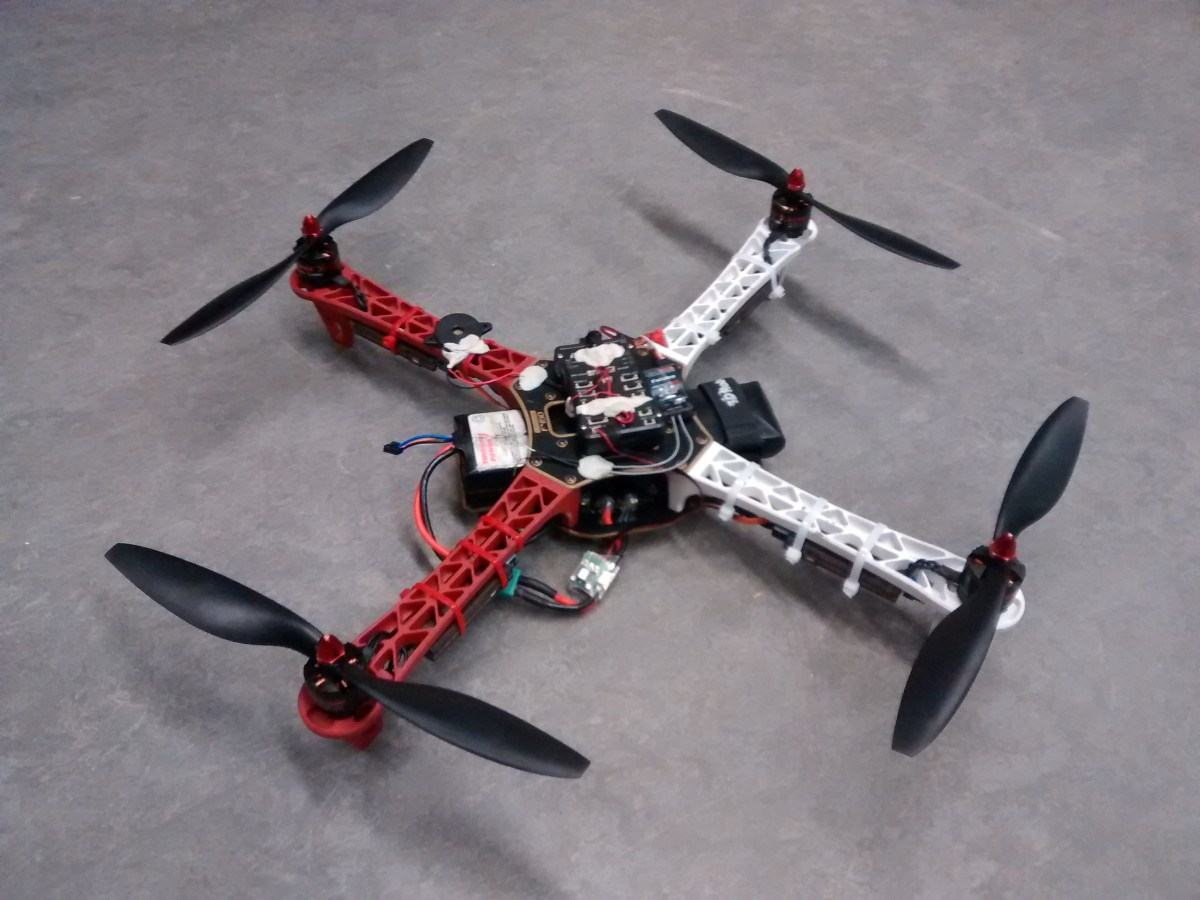
\includegraphics[width=0.6\textwidth]{images/quadrotor.jpg}
	\caption{DJI F450 with Pixhawk v1.5}
\end{figure}





\section*{Software}
\subsection*{Pixhawk Firmware}

\subsection*{Simulator}

\subsection*{AprilTag}







\bibliography{proposal}{}
\bibliographystyle{ieeetr}

\end{document}
